\documentclass[11pt]{article}

%Don't change any thing before \begin{document}
%In fact if you use sth fancy, you might need
%to add more packages, or macros.


\usepackage{../EllioStyle}



\begin{document}
\date{Feb 3, 2020}
\ShortHeadings{Computer Science Theory: Assignment~3}{Elliott Pryor}
\title{CSCI 338: Assignment~3~(6 points)}

\author{Elliott Pryor}


\maketitle

%When writing up your solution, comment out the following until you reach Problem 1.
\noindent
This assignment is due on {\bf Tuesday, March 10, 11:30pm}. It is strongly
encouraged that you use Latex to generate a single pdf file and upload it
under {\em Assignment 3} on D2L. But there will NOT be a penalty for not
using Latex (to finish the assignment). This is {\bf not} a group-assignment,
so you must finish the assignment by yourself.

\section*{Problem 1}

\noindent
Design context-free grammars for the following languages

(1.1) $A=\{a^nb^m|n\neq 2m\}$.

\begin{itemize}
\item $S = aaSb | A | B$
\item $A = aA | a$
\item $B = bB | b$
\end{itemize}


(1.2) $B=\{a^ib^jc^k|i,j,k\geq 0$ and either $i=j$ or $j=k\}$.

\begin{itemize}
\item $S = XC | AY$
\item $A = aA | \epsilon$
\item $C = cC | \epsilon$
\item $X = aXb | \epsilon$
\item $Y = bXc | \epsilon$

\end{itemize}

(1.3) $C=\{a^nb^m|n=3m\}$.

\begin{itemize}
\item $S = aaaSb | \epsilon$

\end{itemize}

(1.4) $D=\{a^nb^m|n\leq m+3\}$.

\begin{itemize}
\item $S = aSb | Sb | A $
\item $A = aaa | aa | a | \epsilon$

\end{itemize}



\newpage
\section*{Problem 2}

\noindent
Decide whether the following grammar is ambiguous.
\newline

$S\rightarrow AB|aaB$

$A\rightarrow a|Aa$

$B\rightarrow b$


\begin{table}[h!]
\begin{tabular}{l r}
S & S\\
AB & aaB\\
AaB & aaB\\
aaB & aaB\\
aab & aab\\
\end{tabular}

\end{table}


There are multiple ways to generate the string ``aab'' with this grammar, so \textbf{yes} the grammar is ambiguous.

\newpage
\section*{Problem 3}

\noindent
Convert the following CFG G to an equivalent PDA.

$R\rightarrow XRX|S$

$S\rightarrow aTb|bTa$

$T\rightarrow XTX|X|\epsilon$

$X\rightarrow a|b$

\begin{figure}[h!]
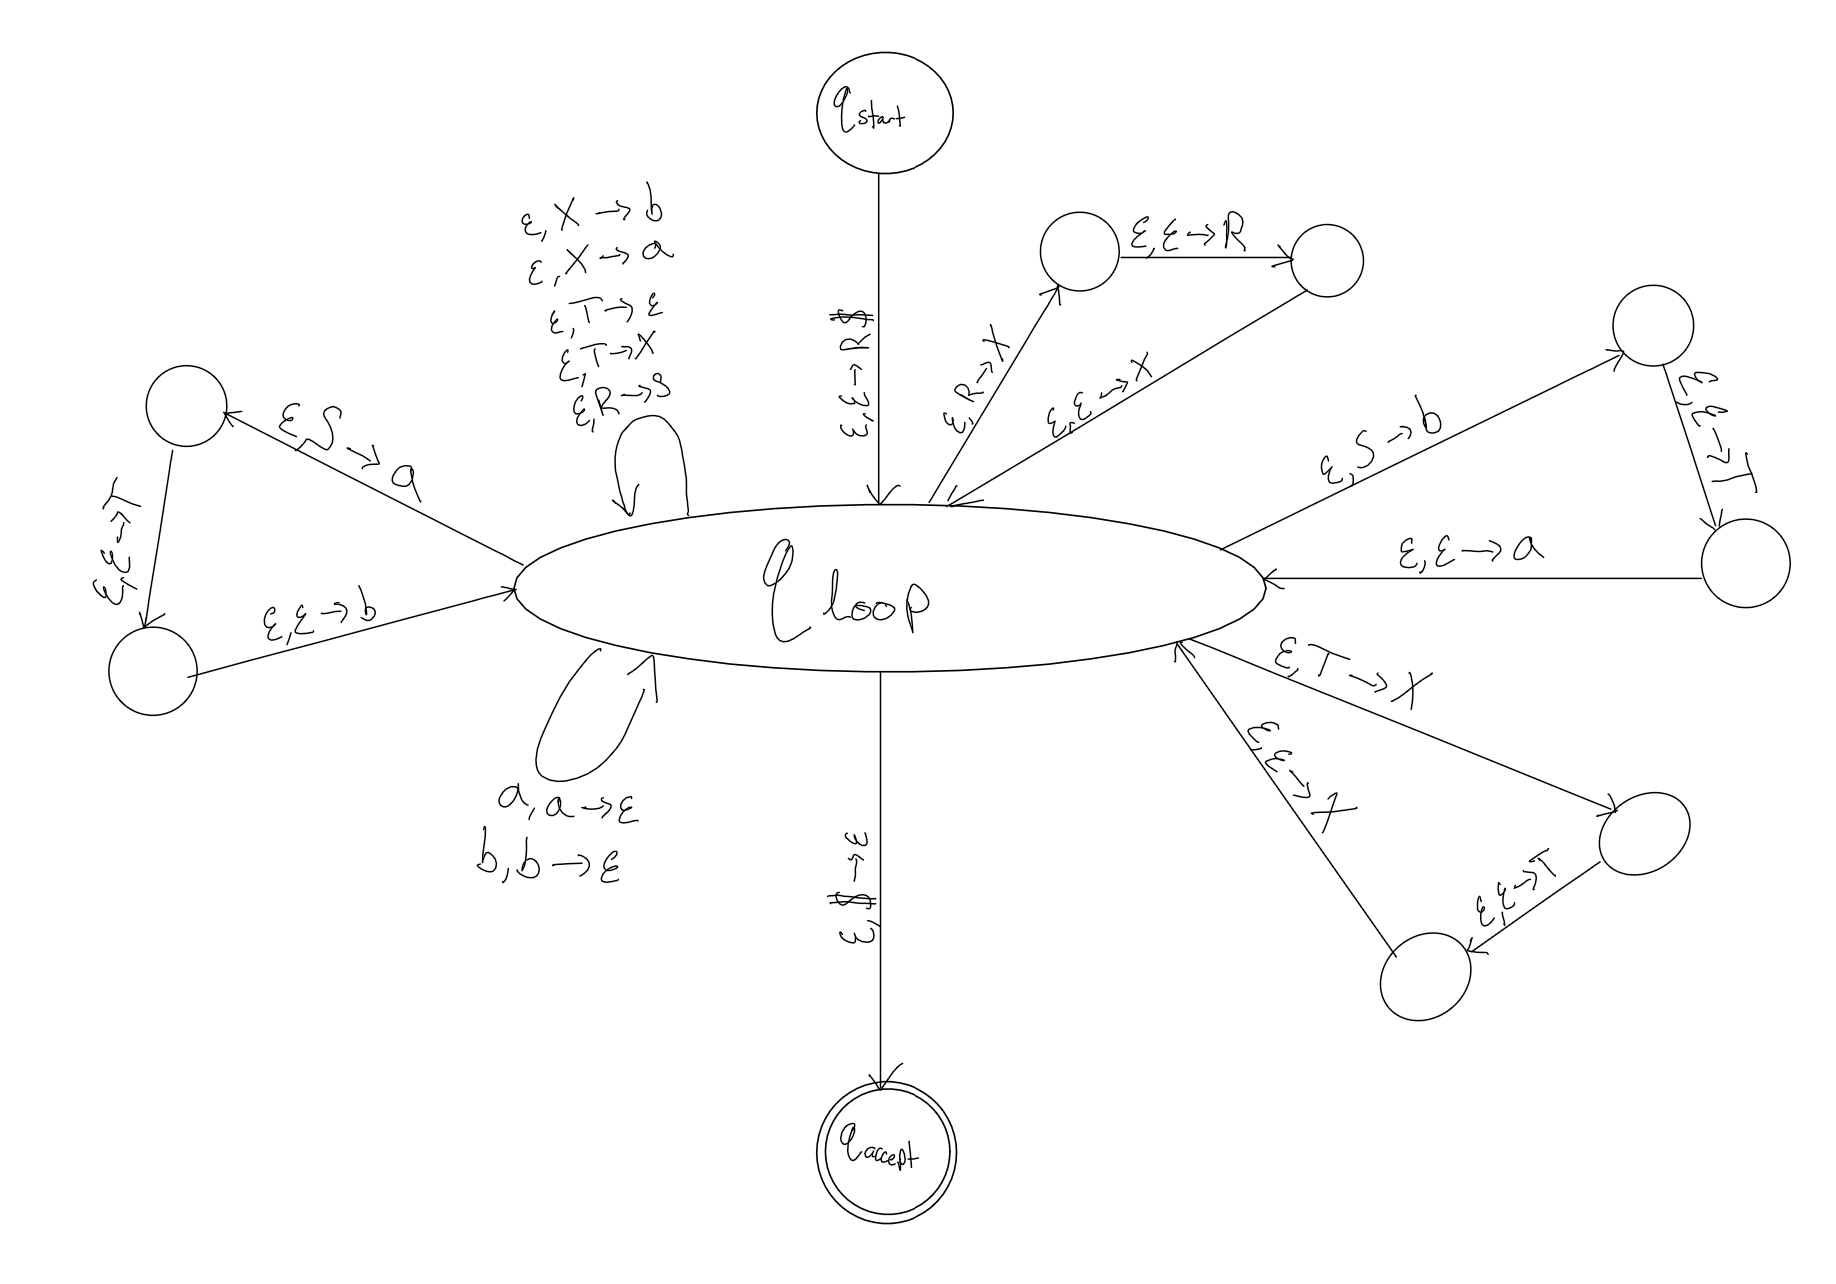
\includegraphics[scale=1]{problem3.png} 
\caption{Solution to Problem 3}
\end{figure}



\newpage
\section*{Problem 4}

\noindent
Let $G=(V,\Sigma,R,S)$ be the following grammar. $V=\{S,T,U\}$;
$\Sigma=\{0,\#\}$; and $R$ is the set of rules:

$S\rightarrow TT|U$

$T\rightarrow 0T|T0|\#$

$U\rightarrow 0U00|\#$

\noindent
(4.1) Describe $L(G)$ in English.
\newline

$L(G)$ has two $\#$'s within a list of an even number of zeros. Or L(G) a single $\#$ one third of the way through a list of zeros with a multiple of three length.

\noindent
(4.2) Prove that $L(G)$ is not regular.


\newpage
\section*{Problem 5}

\noindent
Convert the following CFG into an equivalent CFG in Chomsky Normal Form

$A\rightarrow BAB|B|\epsilon$

$B\rightarrow 00|\epsilon$


$S_0 \rightarrow BD | AB | BA | CC$\\
$A \rightarrow BD | AB | BA | CC$\\
$B \rightarrow CC$\\
$C \rightarrow 0$\\
$D \rightarrow AB$

\newpage
\section*{Problem 6}

\noindent
Using pumping lemma to prove that the following languages are not
context-free.

(6.1) $L=\{a^nb^jc^k|k=nj\}$.
\newline

(6.2) $L=\{a^nb^j|n\geq (j-1)^3\}$.
\newline

\end{document}
